\chapter{Implementation}

This chapter describes how the design was implemented: the project structure, the
technologies used, each module, the deployment procedure and the user interface.

\section{Project Structure}

The project is organised as a monorepo with one directory per service, the ML
pipeline, Kubernetes manifests and the evaluation tooling.

\begin{lstlisting}[basicstyle=\ttfamily\scriptsize]
SecureSME-Platform/
+-- services/
|   +-- ebpf-agent/
|   |   +-- bpf/ids.bpf.c, ids.h     # eBPF kernel program (C, CO-RE)
|   |   +-- loader/ids_loader.c      # libbpf loader, ring buffer -> JSON lines
|   |   +-- ids_agent/               # Python pipeline
|   |   |   +-- collector.py         #   read + normalise kernel events
|   |   |   +-- enrichment.py        #   cgroup -> Pod / container / workload
|   |   |   +-- features.py          #   74 features + behaviour window
|   |   |   +-- detector.py          #   Random Forest + risk scoring
|   |   |   +-- rules.py             #   19 detection rules
|   |   |   +-- shipper.py, metrics.py, __main__.py
|   |   +-- tests/                   # agent unit tests
|   |   +-- Dockerfile               # multi-stage: compile eBPF, Python runtime
|   +-- backend/                     # FastAPI + MongoDB REST API (app/, tests/)
|   +-- frontend/                    # React + Tailwind + Recharts dashboard
+-- ml/
|   +-- generate_dataset.py          # synthetic runtime-telemetry dataset
|   +-- convert_external.py          # BETH / Tetragon -> project schema
|   +-- build_final_dataset.py       # final train.csv / test.csv
|   +-- train_model.py               # training + offline evaluation
|   +-- evaluate_model.py            # test-set evaluation
|   +-- model/                       # ids_model.joblib, evaluation.json
+-- infra/k8s/                       # namespace, MongoDB, backend, frontend, agent
+-- evaluation/                      # victim workload + run_live_eval.py + results
+-- scripts/deploy_minikube.sh       # build images and deploy to minikube
+-- README.md, JOURNAL.md
\end{lstlisting}

\section{Technologies Used}

\begin{table}[H]
\centering
\caption{Technologies used}
\label{tab:tech}
\small
\begin{tabularx}{\textwidth}{>{\raggedright\arraybackslash}p{3.2cm} >{\raggedright\arraybackslash}p{4.0cm} >{\raggedright\arraybackslash}X}
\toprule
\textbf{Layer} & \textbf{Technology} & \textbf{Use} \\
\midrule
Kernel sensor & eBPF, C, clang, libbpf CO-RE, BTF & Tracepoint programs, in-kernel filtering, ring buffer \\
Agent & Python 3.12, NumPy, scikit-learn 1.6, joblib, requests & Enrichment, features, inference, shipping \\
Machine learning & scikit-learn Random Forest, pandas & Training and evaluation \\
Backend & FastAPI, Uvicorn, PyMongo (async), PyJWT, bcrypt & REST API, authentication \\
Database & MongoDB 7.0 & Events, alerts, metrics, users \\
Frontend & React 18, Vite, Tailwind CSS, Recharts, React Router, Axios, lucide-react & Dashboard \\
Platform & Docker, Kubernetes, minikube, kubectl & Packaging and deployment \\
Testing & pytest, Playwright & Unit, API and UI tests \\
Tools & VS Code, Git, GitHub, Ubuntu Linux & Development \\
\bottomrule
\end{tabularx}
\end{table}

\section{Module Description}

\subsection{eBPF Program and Loader}

\textbf{Purpose:} capture security-relevant kernel events with minimal overhead.

\textbf{Implementation highlights:}
\begin{itemize}
    \item One tracepoint handler per system call fills a common event structure
          (\texttt{ids.h}) with cgroup ID, PIDs, UID, process names and arguments.
    \item \texttt{execve} arguments are read on entry and the event is emitted on exit
          only if the call succeeded, so failed executions do not create noise.
    \item File-open events are filtered in the kernel by a list of sensitive path
          prefixes (for example \texttt{/etc/shadow}, \texttt{/var/run/secrets},
          \texttt{/root/.ssh}, runtime sockets).
    \item Events go to a BPF ring buffer; a per-CPU array counts emitted and dropped
          events.
    \item The loader (\texttt{ids\_loader.c}) opens, loads and attaches the CO-RE object
          with libbpf and writes one JSON line per event to standard output. The image is
          built in a multi-stage Dockerfile, so clang and libbpf are not needed on the
          node.
\end{itemize}

\subsection{Python Agent}

\textbf{Purpose:} turn raw kernel events into scored, enriched events and alerts.

\textbf{Implementation highlights:}
\begin{itemize}
    \item \textbf{Collector} starts the loader as a sub-process, reads its JSON lines on a
          thread and normalises them into event dictionaries.
    \item \textbf{K8sEnricher} resolves the cgroup ID to Pod and container and refreshes
          the list of pods on the node from the Kubernetes API.
    \item \textbf{BehaviorTracker} maintains the 60-second window per container and the
          set of known binaries per workload.
    \item \textbf{Detector} loads the model bundle, verifies that the model's feature
          names match the agent's feature module, scores events in batches and combines
          the result with the rules into a decision (Section~5.6).
    \item \textbf{Shipper} sends events and alerts in batches with retries, using the
          shared agent token; \textbf{Metrics} reports CPU, memory, throughput, latency
          and kernel drops every 10 seconds as a heartbeat.
\end{itemize}

Listing~\ref{lst:rules} shows how rules are expressed. Each rule is a small predicate
over the event and its features, with an explicit severity, category and MITRE
technique.

\begin{lstlisting}[language=Python, caption={Excerpt of the rule definitions (\texttt{rules.py})}, label={lst:rules}]
Rule("R001", "Reverse shell command line", "High", "reverse_shell", "T1059.004",
     lambda e, f: f["args_reverse_shell"] and e["event_type"] == "exec"),
Rule("R003", "Service-account token read by a shell tool", "High",
     "credential_access", "T1528",
     lambda e, f: f["ev_open"] and e["path"].startswith(("/var/run/secrets", "/run/secrets"))
     and e["comm"] in TOOLS_FOR_TOKEN_THEFT and not f["ns_system"]),
Rule("R017", "Kubelet / etcd API accessed from a workload", "High",
     "lateral_movement", "T1210",
     lambda e, f: f["ev_connect"] and e.get("dport") in CONTROL_PLANE_PORTS
     and not _platform(f)),
\end{lstlisting}

\subsection{Machine-Learning Pipeline}

\begin{itemize}
    \item \texttt{generate\_dataset.py} creates the labelled synthetic dataset
          (Chapter~4).
    \item \texttt{convert\_external.py} converts BETH and Tetragon data, using all CPU cores
          and an incremental version of the behaviour window that gives identical results
          to the agent's window but in constant time per event.
    \item \texttt{build\_final\_dataset.py} builds \texttt{train.csv} and \texttt{test.csv}
          with the host-based split.
    \item \texttt{train\_model.py} extracts features with the agent's own module, trains the
          Random Forest and writes the model bundle and \texttt{evaluation.json}
          (hold-out, edge cases, unseen template families, 5-fold cross-validation,
          Isolation Forest baseline, latency, feature importance).
    \item \texttt{evaluate\_model.py} reports binary and multi-class metrics, per-source
          results, a threshold sweep and the train/test overlap on any test file.
\end{itemize}

\subsection{Backend (FastAPI)}

The backend exposes the REST API in Table~\ref{tab:api}. Dashboard endpoints require a
JWT obtained from the login endpoint; agent endpoints require the shared agent token.
On start-up the backend creates the MongoDB indexes and the admin user (with a bcrypt
password hash) from the Kubernetes Secret.

\begin{table}[H]
\centering
\caption{REST API endpoints}
\label{tab:api}
\small
\begin{tabularx}{\textwidth}{l >{\ttfamily}l l >{\raggedright\arraybackslash}X}
\toprule
\textbf{Method} & \normalfont\textbf{Path} & \textbf{Auth} & \textbf{Purpose} \\
\midrule
POST  & /api/auth/login & -- & Obtain a JWT \\
GET   & /api/auth/me & JWT & Current user \\
POST  & /api/ingest & Agent token & Batch of events and alerts \\
POST  & /api/agent/heartbeat & Agent token & CPU, memory, latency, drops \\
POST  & /api/agent/evaluation & Agent token & Offline model report \\
GET   & /api/events & JWT & Search / filter events \\
GET   & /api/alerts & JWT & Search / filter alerts \\
GET   & /api/alerts/\{id\} & JWT & Alert details \\
PATCH & /api/alerts/\{id\} & JWT & Acknowledge / resolve \\
GET   & /api/stats & JWT & Overview statistics \\
GET   & /api/namespaces & JWT & Namespaces for filters \\
GET   & /api/agents & JWT & Agent status \\
GET   & /api/evaluation & JWT & Offline and live evaluation \\
POST  & /api/evaluation/live & JWT & Store live evaluation result \\
GET   & /healthz & -- & Liveness / readiness probe \\
\bottomrule
\end{tabularx}
\end{table}

\subsection{Frontend (React Dashboard)}

The dashboard is a single-page React application built with Vite, styled with Tailwind
CSS and charted with Recharts. It is served by nginx, which also proxies
\texttt{/api} to the backend. Its pages are:
\begin{itemize}
    \item \textbf{Login} -- username and password, JWT stored in the browser.
    \item \textbf{Overview} -- kernel events, open alerts, high-severity count, pods
          monitored, agent overhead, detection latency, timeline, severity distribution,
          attack categories, event types, riskiest pods and MITRE techniques.
    \item \textbf{Alerts} -- search and filters (severity, status, namespace, category);
          a detail panel with risk assessment, rules, MITRE technique, Kubernetes context
          and the kernel event; acknowledge and resolve actions.
    \item \textbf{Events} -- live stream of all kernel events with verdict, filters and
          pause.
    \item \textbf{Evaluation} -- live agent overhead and latency, attack-simulation
          results, model benchmarks, confusion matrix, per-category detection and feature
          importance.
\end{itemize}

\section{Deployment}

The complete system is deployed to minikube with the following commands:
\begin{lstlisting}[language=bash]
python3 -m venv .venv && .venv/bin/pip install -r requirements-dev.txt
.venv/bin/python ml/generate_dataset.py && .venv/bin/python ml/train_model.py
minikube start --driver=docker --cpus=2 --memory=3072
./scripts/deploy_minikube.sh        # build images, create Secret, deploy, wait
\end{lstlisting}

The deployment script builds the three images, loads them into minikube, creates the
namespace and a Secret with random credentials, applies the manifests and waits for
the rollouts. Listing~\ref{lst:pods} shows the running system.

\begin{lstlisting}[caption={Running pods and agent start-up log}, label={lst:pods}, basicstyle=\ttfamily\scriptsize]
$ kubectl get pods -A
NAMESPACE     NAME                               READY   STATUS    RESTARTS
ebpf-ids      ids-agent-k5wxf                    1/1     Running   0
ebpf-ids      ids-backend-6bd7986645-qpbtx       1/1     Running   1
ebpf-ids      ids-frontend-6fd6b7f85d-cklvg      1/1     Running   0
ebpf-ids      ids-mongodb-564d7cfdf5-h8d82       1/1     Running   3
ids-demo      shop-web-7b955dcf77-d2pr5          1/1     Running   0
kube-system   coredns-7d764666f9-mgxn8           1/1     Running   4
kube-system   kube-apiserver-minikube            1/1     Running   4
...
$ kubectl -n ebpf-ids logs ds/ids-agent | grep -E "model|ready"
INFO ids.detector: loaded model rf-20261107-161508 (10 classes, threshold 0.50)
INFO ids.collector: eBPF monitor ready: 16 tracepoints attached, 0 failed
\end{lstlisting}

\section{Screenshots}

The following figures show the user interface of the running system in the minikube
cluster.

\begin{figure}[H]
    \centering
    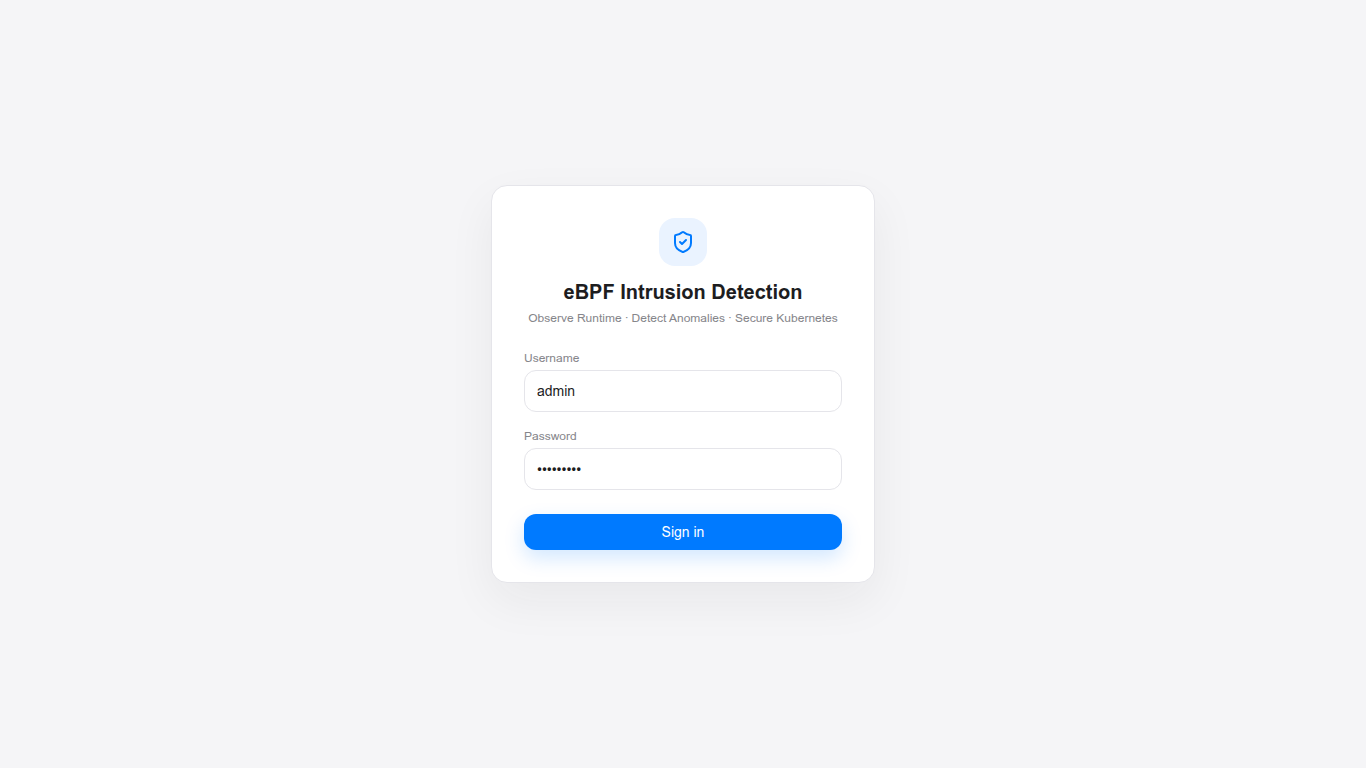
\includegraphics[width=0.82\textwidth]{ss_login.png}
    \caption{Login page}
    \label{fig:ss-login}
\end{figure}

\begin{figure}[H]
    \centering
    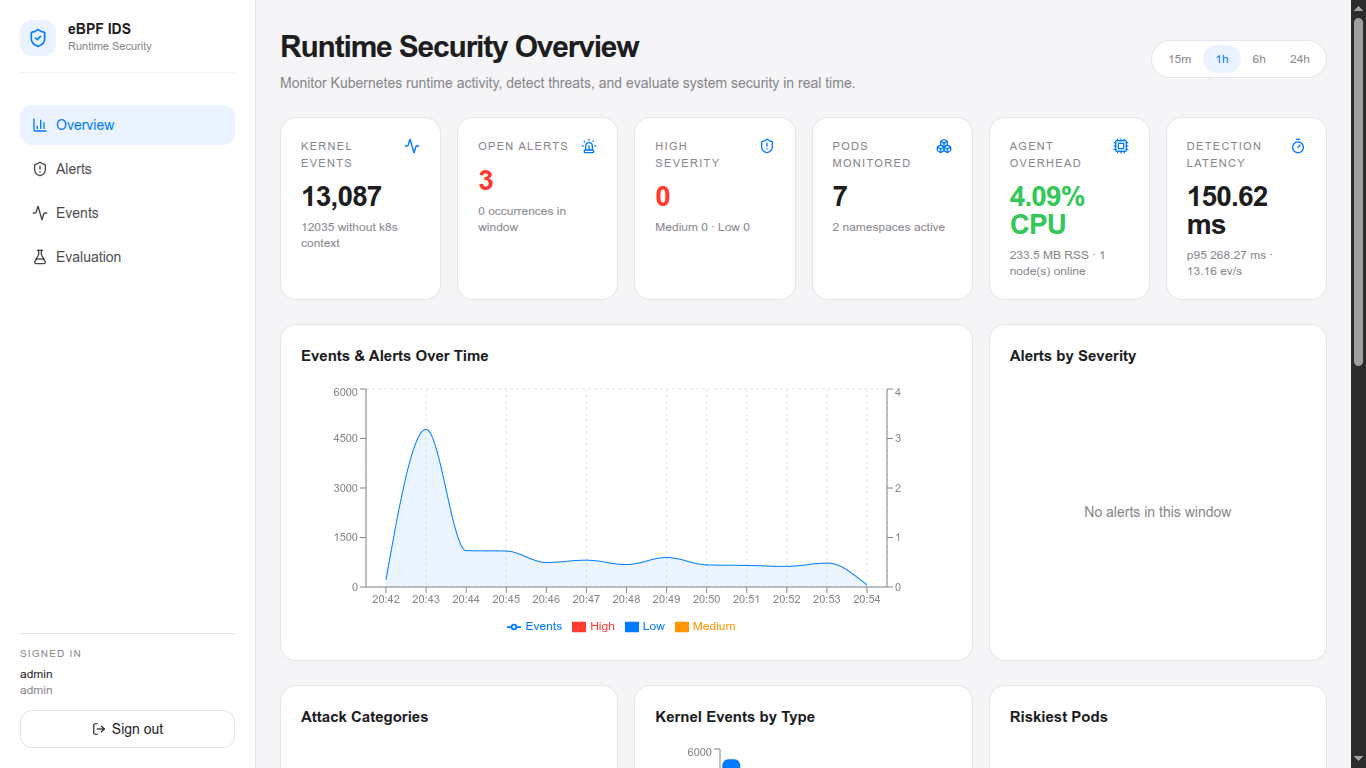
\includegraphics[width=0.95\textwidth]{ss_overview.png}
    \caption{Runtime security overview (top)}
    \label{fig:ss-overview}
\end{figure}

\begin{figure}[H]
    \centering
    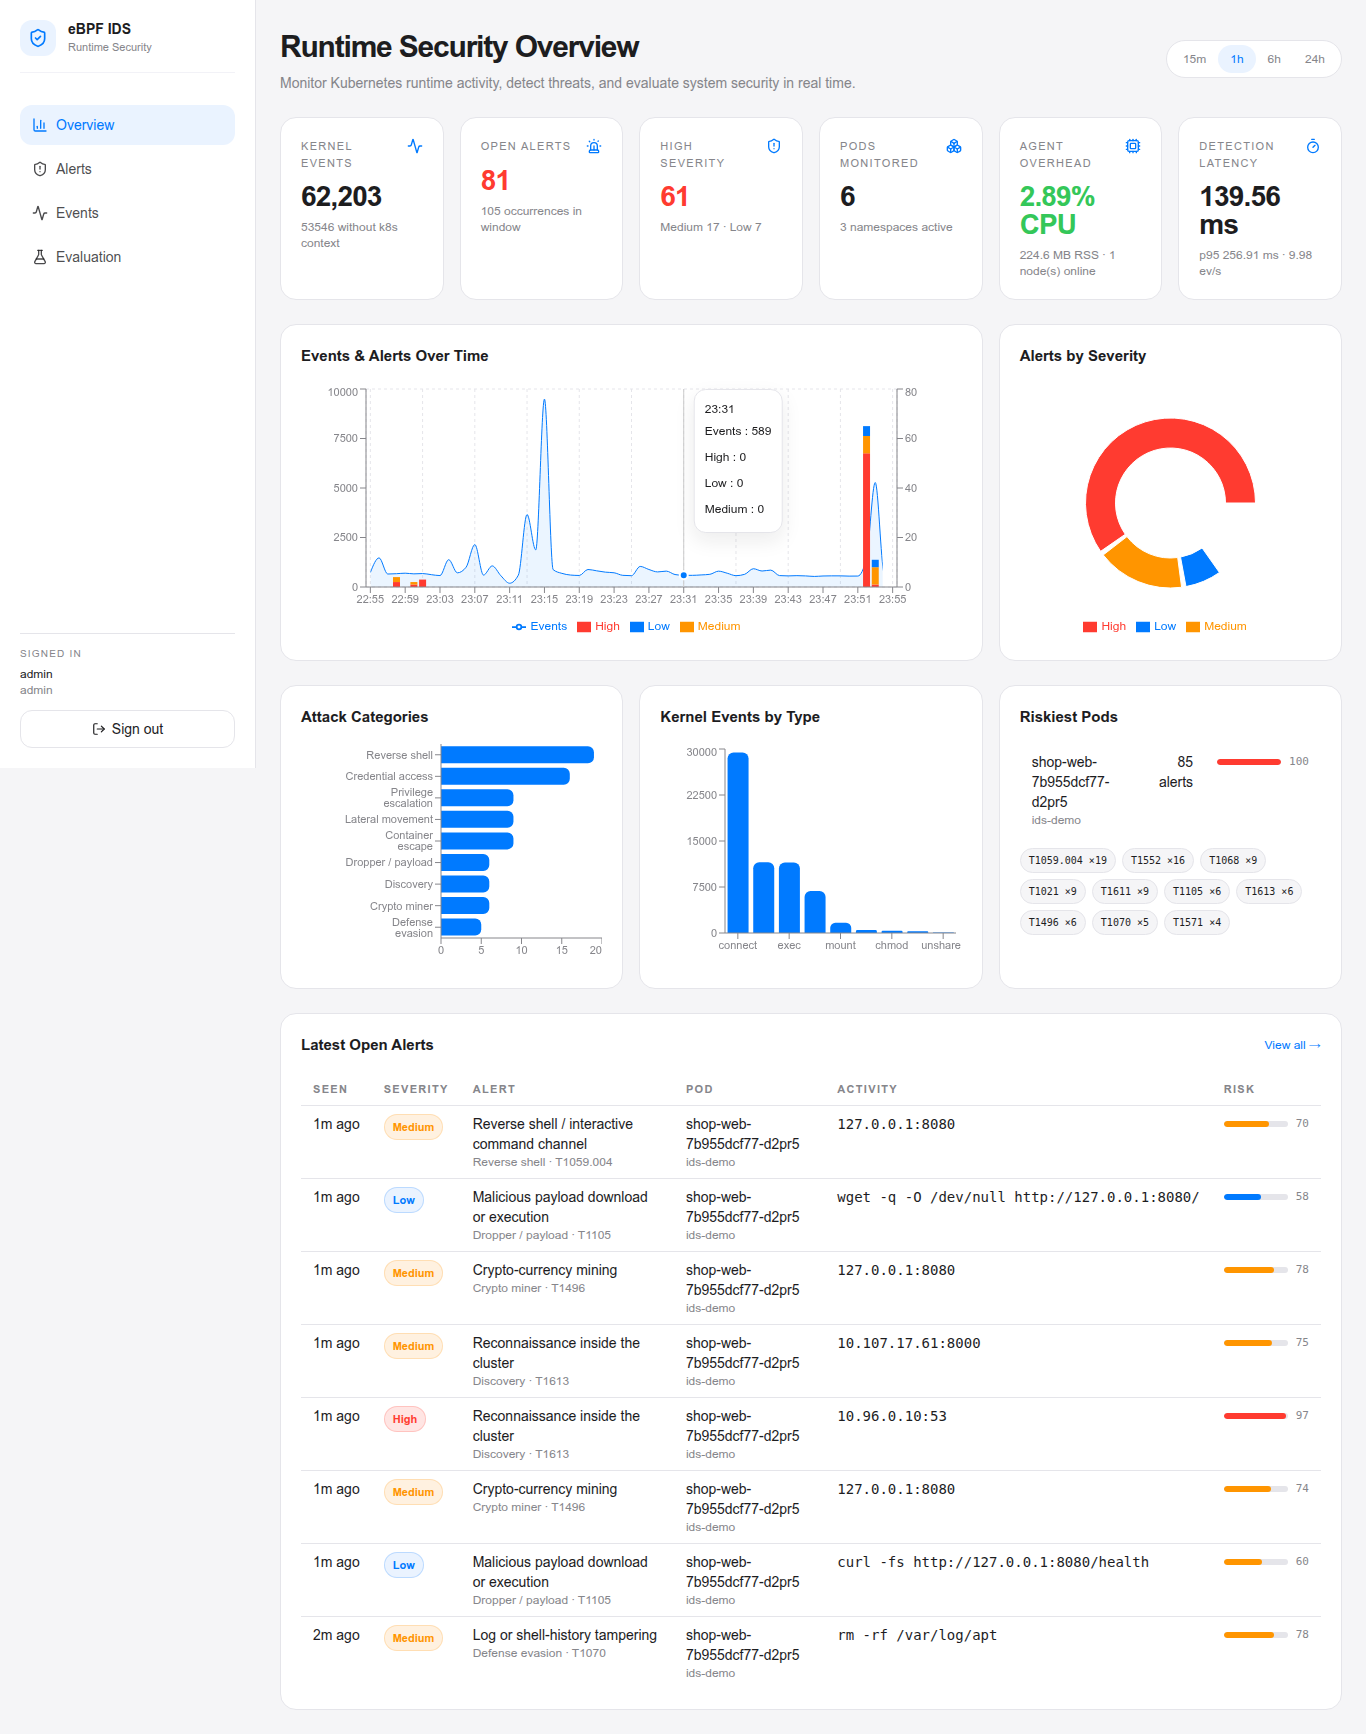
\includegraphics[width=0.8\textwidth]{ss_overview_full.png}
    \caption{Overview after the attack simulation: severities, attack categories,
             kernel event types, riskiest pods with MITRE techniques and latest alerts}
    \label{fig:ss-overview-full}
\end{figure}

\begin{figure}[H]
    \centering
    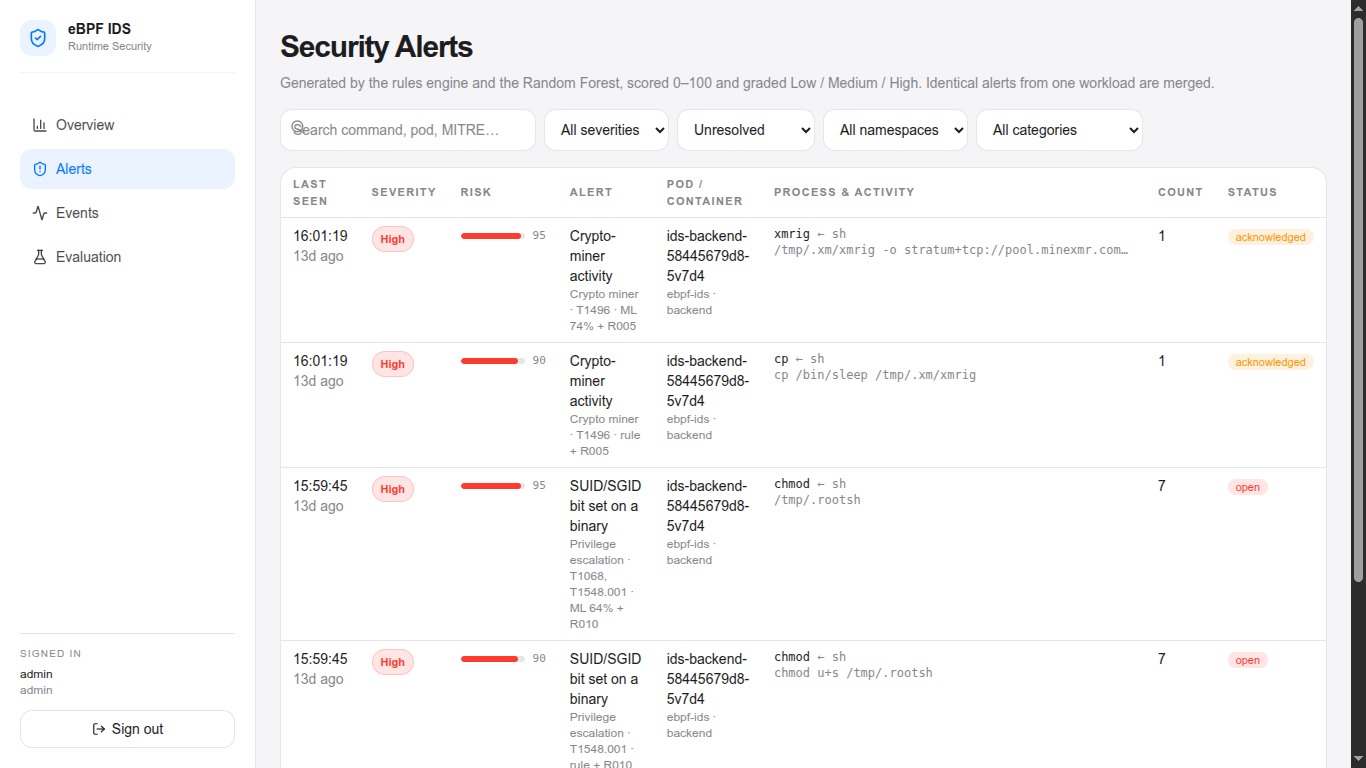
\includegraphics[width=0.95\textwidth]{ss_alerts.png}
    \caption{Security alerts page with risk scores, MITRE techniques and status}
    \label{fig:ss-alerts}
\end{figure}

\begin{figure}[H]
    \centering
    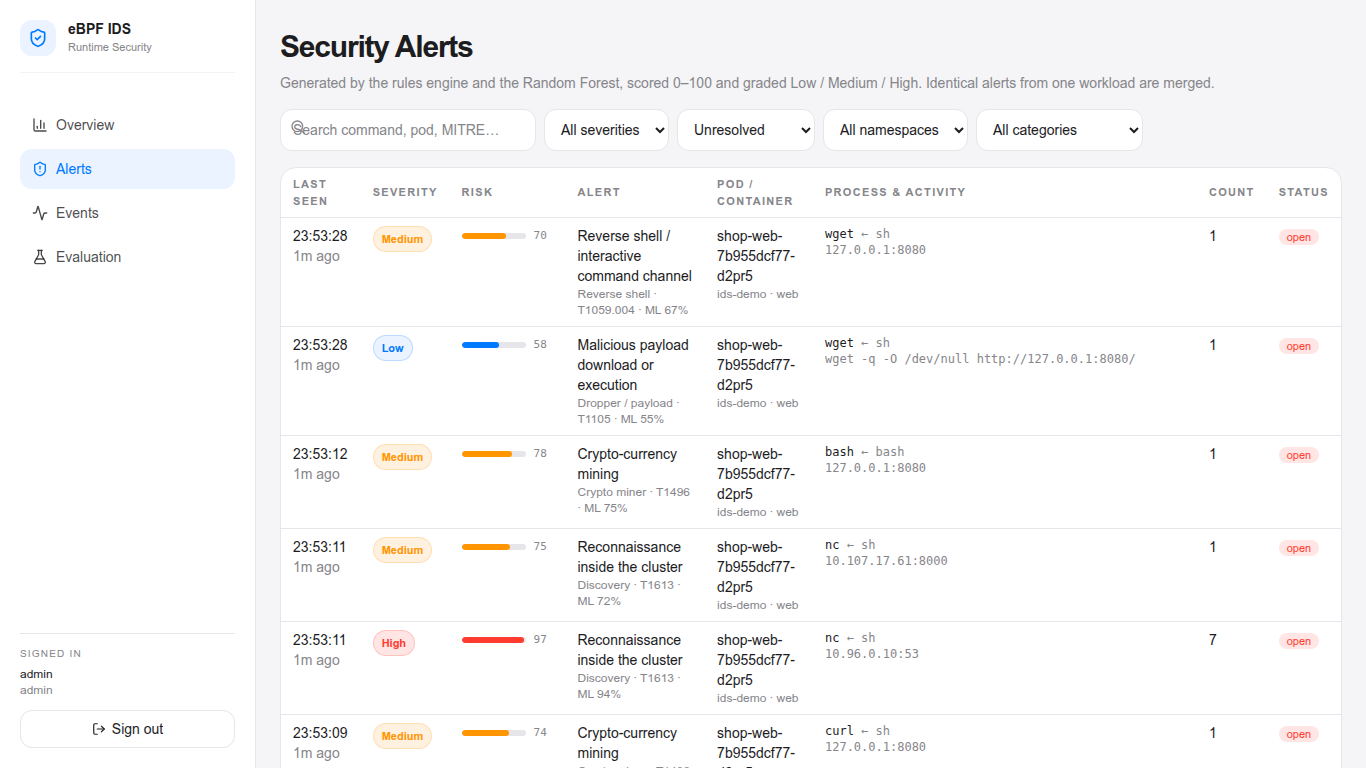
\includegraphics[width=0.95\textwidth]{ss_alerts_live.png}
    \caption{Alerts raised in the test workload \texttt{ids-demo/shop-web}}
    \label{fig:ss-alerts-live}
\end{figure}

\begin{figure}[H]
    \centering
    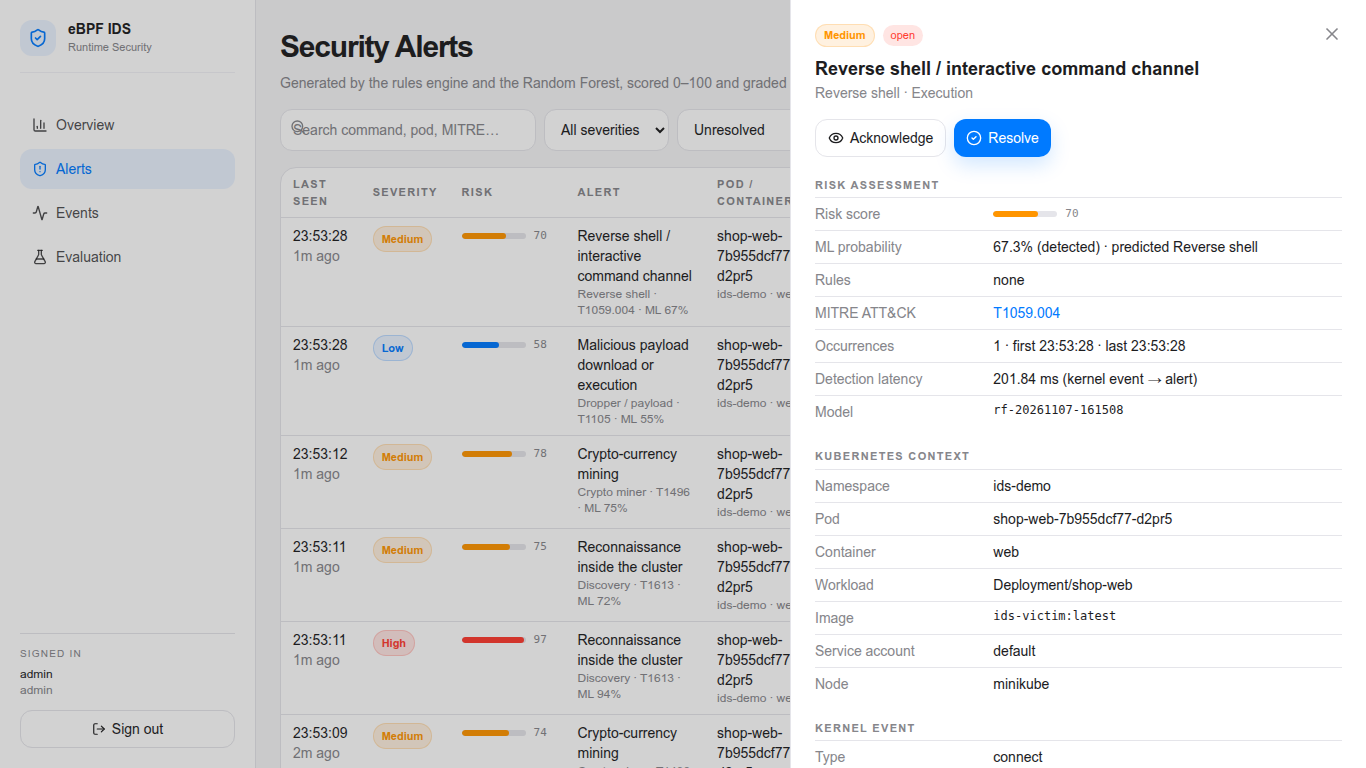
\includegraphics[width=0.95\textwidth]{ss_alert_detail.png}
    \caption{Alert detail panel: risk assessment, ML probability, MITRE technique,
             detection latency and Kubernetes context}
    \label{fig:ss-alert-detail}
\end{figure}

\begin{figure}[H]
    \centering
    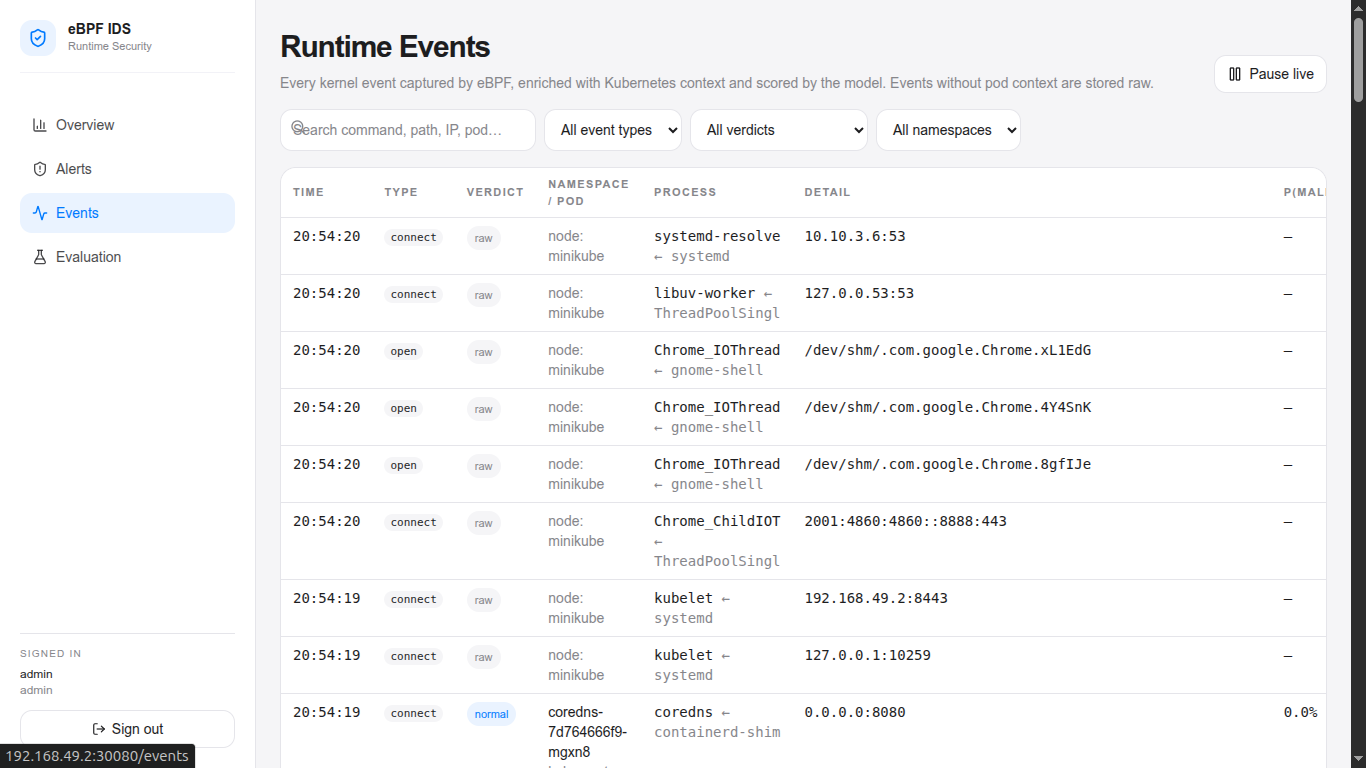
\includegraphics[width=0.95\textwidth]{ss_events.png}
    \caption{Runtime events stream with verdicts}
    \label{fig:ss-events}
\end{figure}

\begin{figure}[H]
    \centering
    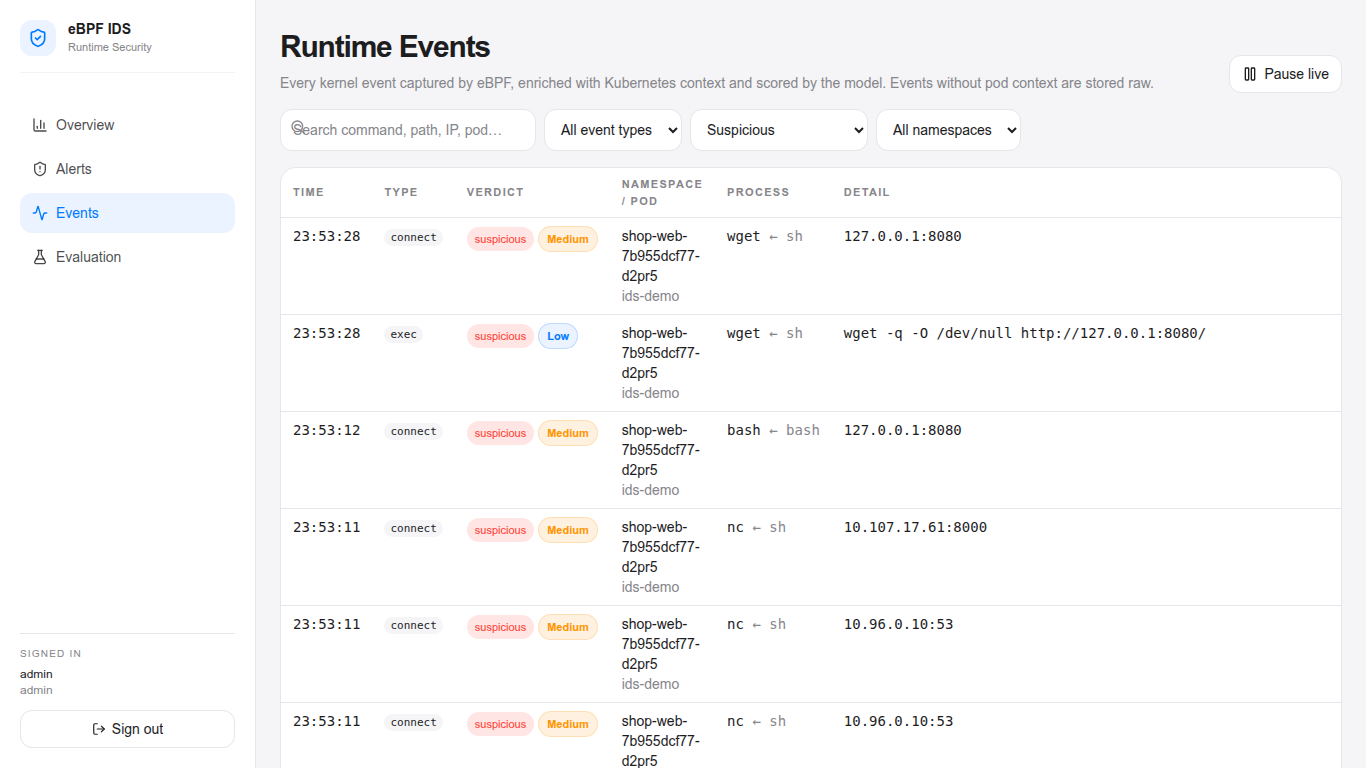
\includegraphics[width=0.95\textwidth]{ss_events_suspicious.png}
    \caption{Events filtered to suspicious verdicts}
    \label{fig:ss-events-sus}
\end{figure}

\begin{figure}[H]
    \centering
    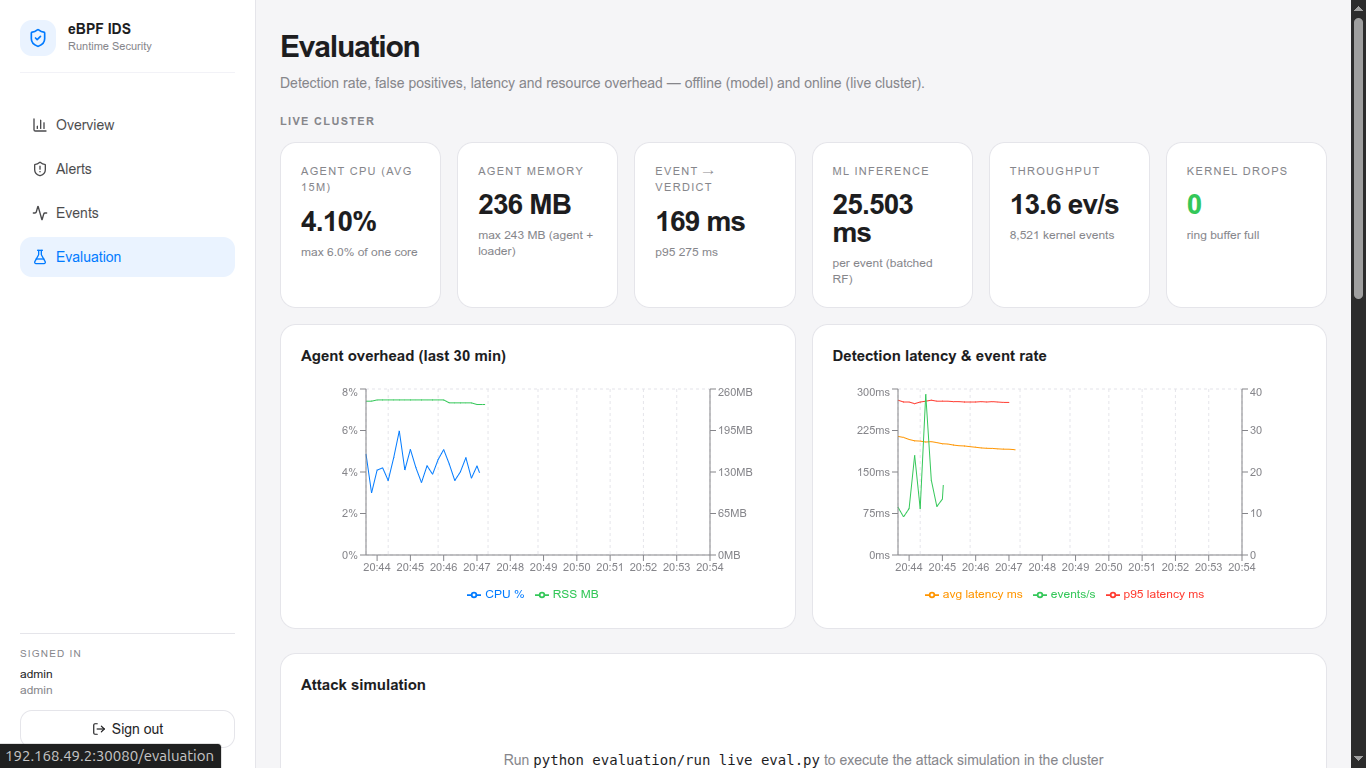
\includegraphics[width=0.95\textwidth]{ss_evaluation_live.png}
    \caption{Evaluation page: live agent overhead, latency and throughput}
    \label{fig:ss-eval-live}
\end{figure}

\begin{figure}[H]
    \centering
    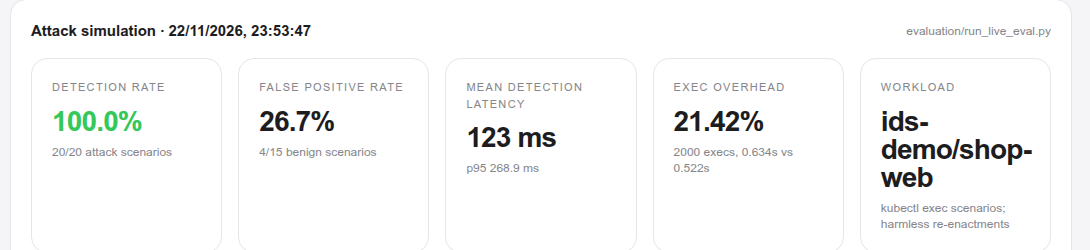
\includegraphics[width=0.95\textwidth]{ss_attack_simulation.png}
    \caption{Evaluation page: attack-simulation summary}
    \label{fig:ss-attack-sim}
\end{figure}

\begin{figure}[H]
    \centering
    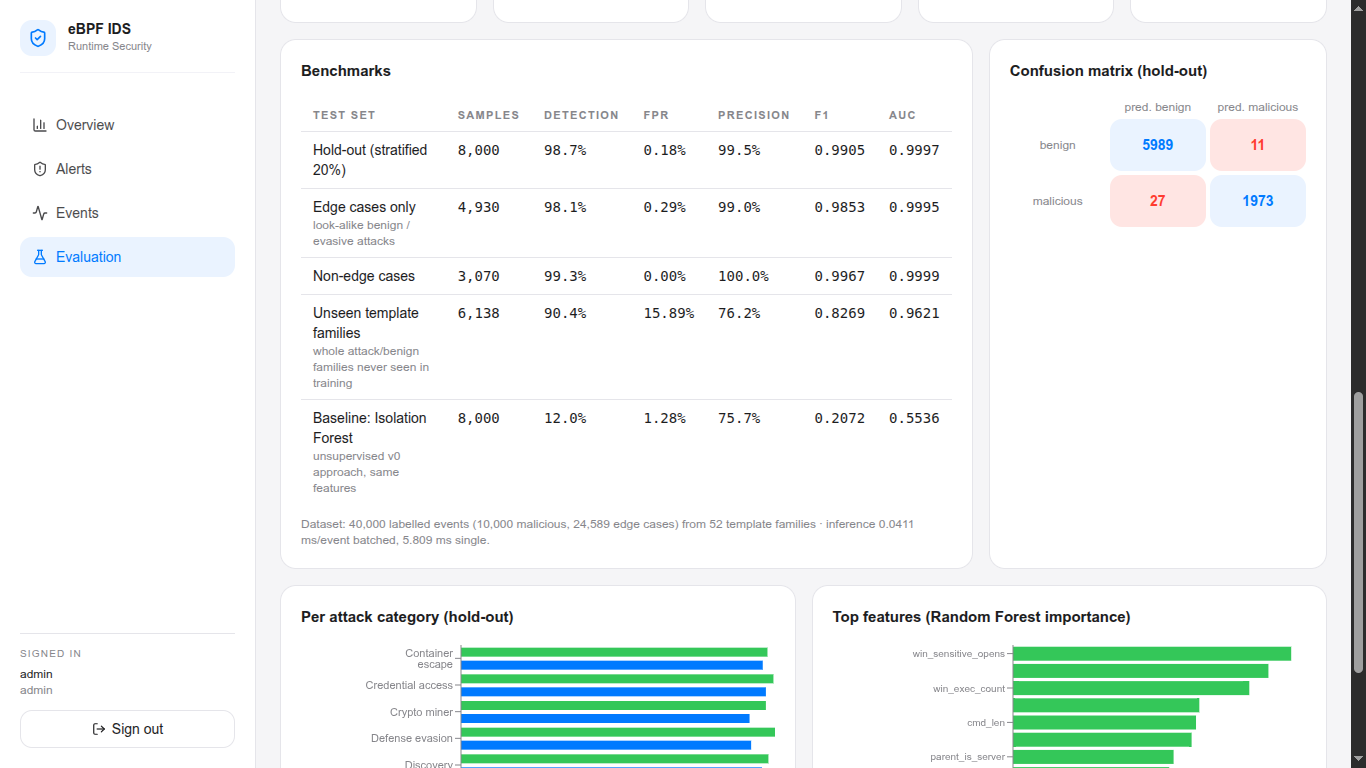
\includegraphics[width=0.95\textwidth]{ss_evaluation_model.png}
    \caption{Evaluation page: offline model benchmarks and confusion matrix}
    \label{fig:ss-eval-model}
\end{figure}

\begin{figure}[H]
    \centering
    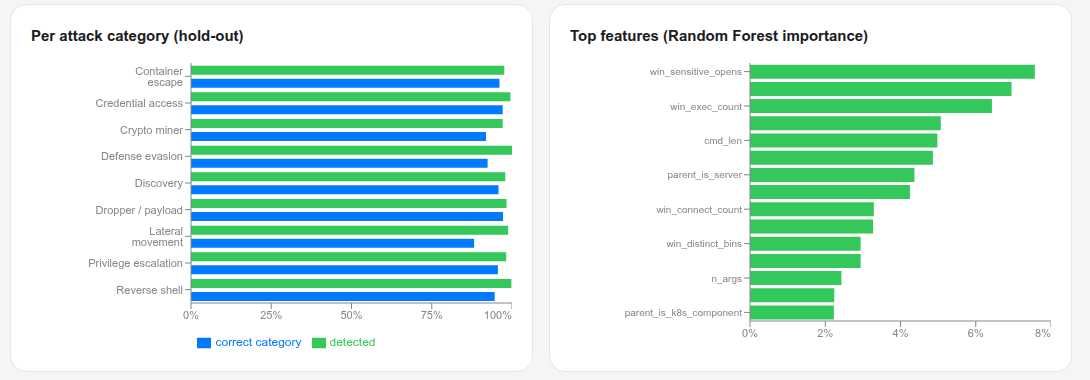
\includegraphics[width=0.95\textwidth]{ss_eval_categories.png}
    \caption{Evaluation page: per-category detection and feature importance}
    \label{fig:ss-eval-cat}
\end{figure}
